% !TEX encoding = UTF-8
% !TEX TS-program = pdflatex
% !TEX root = ../tesi.tex

%**************************************************************
\chapter{Progettazione e codifica}
\label{cap:progettazione-codifica}
%**************************************************************

\intro{In questo capitolo verranno spiegate le tecnologie utilizzate per lo sviluppo e l'architettura del prodotto software}\\

%**************************************************************
\section{Tecnologie e strumenti}
\label{sec:tecnologie-strumenti}

Di seguito viene data una panoramica delle tecnologie e strumenti utilizzati per lo sviluppo delle maschere e per la collaborazione con i colleghi stagisiti ed il tutor aziendale.

\subsection{Tecnologie}
\label{subsec:tecnologie}

\subsubsection{Vue.js}
\label{subsubsec:vue.js}

\begin{figure}[H]
	\begin{center}
		
\includegraphics[width=0.7\columnwidth]{vue.png}
		\caption{Logo di Vue.js}
	\end{center}
\end{figure}
Vue.js è un framework javascript open source nato nel 2013 che presenta un'architettura adottabile in modo incrementale che si concentra sulla composizione dei componenti, inoltre sono presenti funzionalità avanzate offerte tramite librerie e pacchetti di supporto. I componenti Vue estendono gli elementi HTML di base per incapsulare del codice riutilizzabile quindi a livello generale i componenti sono elementi personalizzati a cui il compilatore Vue associa una particolare funzionalità.\\
Vue utilizza quindi una sintassi basata su HTML e consente di associare il DOM renderizzato ai dati dell'istanza di Vue sottostante. In questo modo i modelli Vue possono essere analizzati da browser e parser HTML conformi alle modifiche ed inoltre con il sistema di reattività Vue è in grado di calcolare il numero minimo di componenti per eseguire nuovamente il rendering applicando la quantità minima di manipolazioni DOM quando cambia lo stato dell'app. Vue presenta un sistema reattivo grazie all'utilizzo di oggetti semplici Javascript ed ad un re-rendering ottimizzato: ogni componente durante il render tiene traccia delle sue dipendenze in modo tale che il sistema sappia quando e di quali componenti deve effettuare nuovamente il render.\\
Un problema che afflige le \gls{web applicationg} a pagina singola è che forniscono agli utenti la risposta basata solamente sull'URL dal server, di conseguenza l'utilizzo dei segnalibri a determinate schermate e la condivisione dei collegamenti a sezioni specifiche risulta molto difficile se non impossibile. Vue.js per riuscire a risolvere questo problema fornisce un'interfaccia, detta router, che modifica ciò che viene visualizzato sulla pagina in base all'URL corrente, indipendentemente da come è stato modificato. Infatti Vue.js viene fornito con il pacchetto open source "vue-router" che fornisce un'API per aggiornare l'URL dell'applicazione, supportare la cronologia di navigazione e le reimpostazioni di email e password. Tramite questa tipologia di router i componenti devono essere mappati alla route a cui appartengono per indicare dove deve essere eseguito il loro render.\\
Questo framework implementa il pattern MVVM, acronimo per Model-View-View-Model, una declinazione del più famoso MVC, ovvero Model-View-Controller. I componenti del MVVM sono:
\begin{itemize}
	\item Model (o Modello): l'implementazione del dominio dati come per il classico Modello del pattern MVC;
	\item View (o Vista): il componente grafico renderizzato dall'utente formato da HTML e CSS;
	\item ViewModel (o Vista per il Modello): il collante tra gli altri due componenti, esso fornisce alla View i dati in formato consono alla rappresentazione ed il comportamento di alcuni elementi dinamici.
\end{itemize}
La grossa differenza tra il pattern implementato da Vue.js e il Model-View-Controller sta nella differenza tra Controller e ViewModel. Il primo, infatti, è una porzione di codice che gestisce la logica di business grazie al Model e ritorna una View da mostrare all'utente; il secondo, invece, rappresenta una versione parallela al Model che risulta essere legato alla View e descrive il comportamento di quest'ultima con funzioni associate. Quindi mentre il Controller esegue logiche di business prima del rendering della View, il ViewModel definisce il comportamento dell'applicazione a runtime.

\subsubsection{Vuetify}
\label{subsubsec:vuetify}

Vuetify è un \gls{frameworkg} UI completo costruito su Vue.js nel 2014 ed il suo obiettivo è fornire agli sviluppatori gli strumenti per poter creare esperienze utente ricche e coinvolgenti. A differenza di altri framework Vuetify è progettato da zero in modo tale da renderlo facile da imparare ed essere gratificante da padroneggiare con centinaia di componenti realizzate dalle specifiche di Material Design.\\
Un pregio di questo \gls{frameworkg} è che adotta un approccio al mobile, questo significa che la \gls{web applicationg} sviluppata tramite esso sarà pienamente utilizzabile immediatamente su un tablet, un telefono ed un computer. Inoltre è un \gls{frameworkg} in sviluppo attivo che viene aggiornato settimanalmente rispondendo ai problemi e relativi report della community. Un altro pregio è, come si può vedere nell'immagine sottostante, il gran numero di funzionalità che possiede Vuetify in confronto agli altri framework di Vue.
\begin{figure}[H]
	\begin{center}
		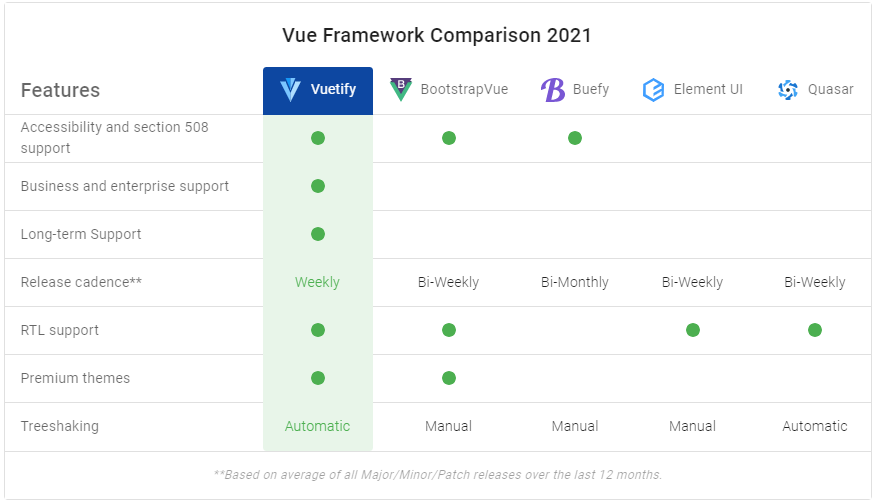
\includegraphics[width=1\columnwidth]{vuetify.png}
		\caption{Funzionalità di Vuetify}
	\end{center}
\end{figure}

\subsubsection{Vuex}
\label{subsubsec:vuex}

Vuex è una libreria  per applicazioni sviluppate in Vue.js e serve come store centralizzato per tutti i componenti dell'applicazione. Esso contiene stati e regole che assicurano che lo stato può essere modificato solo in modo prevedibile.\\
Inoltre Vuex è uno state management pattern che aiuta a salvare i dati in maniera persistente per poterli utilizzare all'interno dell'applicazione da diversi componenti in maniera efficiente.
\begin{figure}[H]
	\begin{center}
		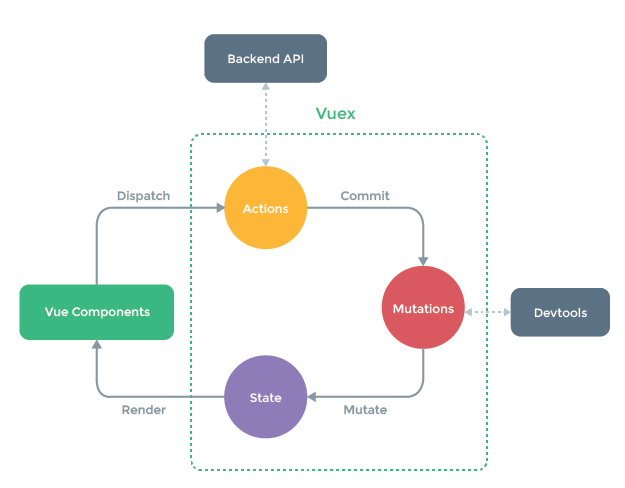
\includegraphics[width=0.7\columnwidth]{vuex.png}
		\caption{Pattern di Vuex}
	\end{center}
\end{figure}

\subsection{Strumenti}
\label{subsec:strumenti}

\subsubsection{Github}
\label{subsubsec:github}

Github è un servizio web e cloud-based fondato nel 2008 che aiuta gli sviluppatori ad archiviare, gestire il codice, tracciare e controllare le modifiche. I due argomenti principali legati a Github sono: controllo versioni e Git.\\
Il controllo versioni aiuta a tracciare e gestire le modifiche del codice di un progetto software: più un progetto risulta essere di grandi dimensioni più il controllo delle versioni diventa fondamentale. Infatti questo aiuta gli sviluppatori a lavorare con sicurezza attraverso due azioni:
\begin{itemize}
	\item branching: uno sviluppatore duplica parte del codice sorgente, detto repository, in modo da apportare modifiche in modo sicuro senza influenzare l'intero progetto;
	\item merging: una volta che lo sviluppatore è certo di aver prodotto del codice funzionante può fondere quel codice nel quello sorgente e renderlo ufficiale.
\end{itemize}
In questo modo tutte le modifiche possono essere monitorate e, se necessario, ripristinate. Inoltre grazie a questi concetti è possibile lavorare sullo stesso progetto in diversi sviluppatori senza problemi di ripetizioni di codice o conflitti durante lo sviluppo.\\
Git è un sistema di controllo versioni distribuito realizzato nel 2005, ovvero l'intero codice base e la cronologia sono disponibili sul computer di ogni sviluppatore. In questo modo è possibile creare facilmente ramificazioni e fusioni.\\
Per organizzare il lavoro abbiamo creato un'\textit{organization}, prodotto offerto da Github che rende più semplice la collaborazione su più progetti contemporaneamente. Infatti ogni stagista ha creato la propria repository all'interno di questo spazio comune in modo tale da lavorare con i colleghi contemporaneamente e dare la possibilità ai tutor aziendali di visionare il lavoro svolto.

\subsubsection{Figma}
\label{subsubsec:figma}

Figma è uno strumento nato nel 2016 rivolto ai web designer che hanno bisogno di un tool per la progettazione di interfacce. I vantaggi offerti da questo strumento sono i seguenti:
\begin{itemize}
	\item accessibilità multipiattaforma
	\item sistema di collaborazione in real-time
	\item utilizzo degli strumenti responsive oriented per una progettazione ottimale
	\item lavora in vettoriale
\end{itemize}
Grazie a questo strumento io e gli altri stagisti legati all'ambito \gls{front endg} abbiamo potuto creare dei prototipi delle maschere che avremmo dovuto sviluppare.

\subsubsection{Stoplight}
\label{subsubsec:stoplight}

Stoplight è una piattaforma di progettazione \gls{api} collaborativa che si integra perfettamente nei flussi di lavoro per consentire a chiunque lavori con le \gls{api} di essere più produttive. Questa piattaforma si basa su tre principi guida fondamentali, in modo da essere responsabili, collaborativi e con intenti positivi. I principi sono i seguenti:
\begin{itemize}
	\item quando si vede un'opportunità per avere un impatto, bisogna coglierla;
	\item bisogna confidare l'uno nell'altro per aggiungere valore e risolvere problemi attraverso il lavoro di squadra;
	\item bisogna cercare di capire gli altri ascoltando, indagando e rispondendo con attenzione.
\end{itemize}
Grazie a questa piattaforma si può aiutare gli utenti interni ed esterni ad integrarsi rapidamente alll'\gls{api} di un altro utente pubblicando documentazione interattiva, tutorial ed esempi di codice sempre aggiornati.\\
Noi stagisti abbiamo utilizzato questo strumento per non far dipendere lo sviluppo del \gls{front endg} con quello del \gls{back endg} e quindi riuscire a sviluppare in parallelo le due parti ed effettuare l'integrazione tra le due solo dopo esserci assicurati di avere il lavoro quasi concluso e poterci concentrare sulla risoluzione di possibili problemi in integrazione.

\subsubsection{Visual Studio Code}
\label{subsubsec:visual-studio-code}

Visual Studio Code è un editor di codice sorgente sviluppato da Microsoft nel 2015. Esso può essere utilizzato con diversi linguaggi di programmazione, infatti incorpora in esso diverse funzioni che variano dal linguaggio con cui si sta programmando. Un punto di forza di questo editor è la sua grande malleabilità, infatti l'utente può installare o disinstallare diversi plugin in funzione del linguaggio che sta utilizzando.\\
Un altro punto di forza è la sua integrazione con Git facilitando il controllo di versione del lavoro svolto dal programmatore che ha la possibilità di controllare le modifiche fatte, risolvere eventuali conflitti e salvare il lavoro nella repository. Altri punti di forza di questo editor sono i seguenti:
\begin{itemize}
	\item IntelliSense, estensione che fornisce suggerimenti di completamento per variabili, metodi e moduli. In particolare per i metodi fornisce una breve spiegazione dei parametri che accettano e del loro funzionamento;
	\item Debug semplificato grazie ai plugin messi a disposizione e all'interfaccia grafica intuitiva;
	\item Modifica veloce delle righe di codice grazie ad avvisi su codice sospetto, possibilità di selezionare più righe contemporaneamente e suggerimenti sui parametri;
	\item Navigazione e refactoring del codice semplice.
\end{itemize}

\section{Organizzazione dei file}
\label{sec:organizzazione-file}

Quando si crea un progetto per la prima volta tramite il \gls{frameworkg} Vue.js vengono create di default delle cartelle e dei file per facilitare la progettazione del software. La suddivisione delle cartelle è rappresentata qui di seguito.

\begin{lstlisting}[caption=Organizzazione dei file., label=lst::orgFile]
	|-- front-end-vue
	|-- codice
	|   |-- .editorconfig
	|   |-- .eslintignore
	|   |-- .eslintrc.js
	|   |-- .gitignore
	|   |-- .prettierc.json
	|   |-- .prettierignore
	|   |-- babel.config.js
	|   |-- jest.config.js
	|   |-- jsconfig.json
	|   |-- package-lock.json
	|   |-- package.json
	|   |-- README.md
	|   |-- vue.config.js
	|   |-- .vscode
	|   |-- coverage
	|   |-- dist
	|   |-- pubblic
	|   |-- src
	|   |   |-- App.vue
	|   |   |-- main.js
	|   |   |-- style.css
	|   |   |-- assets
	|   |   |-- components
	|   |   |-- plugins
	|   |   |-- router
	|   |   |-- store
	|   |   |   |-- index.js
	|   |   |   |-- modules
	|   |   |-- view
	|   |-- tests
	|       |-- unit
	|-- docs
	|-- documento tecnico
	|-- directoryList.md
\end{lstlisting}

La cartella principale si chiama \textbf{\textit{front-end-vue}} ed essa contiene i file di configurazione del progetto, il file \textbf{\textit{readme}}, il file di \textbf{\textit{gitignore}} ed il file \textbf{\textit{directoryList.md}}, creato automaticamente attraverso il comando \textit{mddir} dove viene scritta la struttura delle cartelle del progetto. Inoltre sono presenti tre cartelle:
\begin{itemize}
	\item \textbf{\textit{codice}}, contenente il codice del progetto;
	\item \textbf{\textit{docs}}, contenente file YAML utilizzato per la configurazione di Stoplight;
	\item \textbf{\textit{documento tecnico}}, contente i file latex utilizzati per la stesura di questo documento.
\end{itemize} 
Per quanto riguarda la cartella legata al codice, essendo la più importante, necessita di una spiegazione degli elementi che la contengono. I file e le sottocartelle create automaticamente alla creazione del progetto però non verranno spiegate, mentre i restanti elementi sono i seguenti:
\begin{itemize}
	\item \textbf{\textit{coverage}}: cartella che contiene i file e le cartelle create automaticamente quando vengono fatti partire i test di unità;
	\item \textbf{\textit{src}}: cartella in cui sono presenti file e cartelle necessari per il funzionamento del progetto e sono:
	\begin{itemize}
		\item il file \textbf{\textit{App.vue}} è la radice dell'applicazione definita nel formato Vue Component e di solito serve a definire il modello della pagina;
		\item il file \textbf{\textit{Main.js}} di tipo javascript che inizializza il file \textit{App.vue} ed è responsabile dell'impostazione dei plugin e dei componenti di terze parti da utilizzare per lo sviluppo dell'applicazione;
		\item la cartella \textbf{\textit{assets}} contenente le immagini utilizzate all'interno del sito, come quella del logo;
		\item la cartella \textbf{\textit{components}} contenente la barra di navigazione (navbar) e le varie finestre d'avviso;
		\item la cartella \textbf{\textit{plugins}} contenente i file javascript dei plugin utilizzati per lo sviluppo, in questo caso di Vuetify;
		\item la cartella \textbf{\textit{router}} contenente un omonimo file javascript dove vengono definite le route ovvero le varie pagine in cui può navigare l'utente;
		\item la cartella \textbf{\textit{store}} contenente i file per la configurazione delle chiamate al database e lo state management;
		\item la cartella \textbf{\textit{view}} contenente le possibili schermate che può visualizzare l'utente;
		\item la cartella \textbf{\textit{tests}} che contiene la sottocartella \textbf{\textit{unit}} dove sono presenti i test di unità effettuati.
	\end{itemize}
\end{itemize}

\textit{Nelle sezioni di seguito verranno spiegate in dettaglio il funzionamento delle chiamate al back end e delle varie maschere implementate con le loro criticità}

\section{Chiamate al back end}
\label{sec:chiamate-back-end}

Il file principale, \textbf{\textit{index.js}}, contiene la configurazione di Vuex e del persisted state con l'inclusione dei moduli che sono di numero tanti quanti sono i servizi del \gls{back endg} che vanno ad invocare. Per rendere più chiaro ed efficiente il lavoro ho creato quindi il file \textbf{\textit{CurrentUser.js}}, legato al servizio del back end dell'utente, e il file \textbf{\textit{NftService.js}}, legato al servizio del back end degli NFT.\\
Entrambi i file hanno la struttura uguale e quello che cambia è il contenuto, infatti sono caratterizzati da quattro elementi costanti:
\begin{itemize}
	\item state, contenente le risorse che verranno utilizzate nei metodi;
	\item actions, contenente i metodi dove vengono fatte le invocazioni ai servizi del backend tramite axios;
	\item mutations, contenente i metodi che modificano le risorse, sono come un equivalente dei metodi set;
	\item getters, contenente i metodi che ritornano i valori presenti nelle risorse.
\end{itemize}

Gli state del file \textbf{\textit{CurrentUser.js}} li ho resi persistenti, in questo modo potranno essere utilizzati all'interno della \gls{web applicationg}, per esempio dopo che l'utente ha eseguito l'autenticazione utilizzo i suoi dati per visualizzare il suo nome nel bottone che lo porta alla pagina personale. Queste informazioni possono essere utilizzate per fare dei controlli che decidono se reindirizzare o meno certe parti della \gls{web applicationg}.\\
Essendo legati a servizi diversi i metodi e le chiamate al \gls{back endg} dei due file sono molto diversi e nelle sezioni successive verranno spiegate nel dettaglio.

\subsection{CurrentUser.js}
\label{subsec:currentuser}

In questo file ho implementato diversi servizi legati all'utente. I servizi in questione sono:
\begin{itemize}
	\item \textbf{Autenticazione}:
	\begin{lstlisting}[caption=Autententicazione., label=lst::autenticazione]
		loginUser({ commit }, user) {
			axios
			.post(urlBackEnd + 'login', {
				email: user.email,
				password: user.password
			})
			.then(response => {
				commit('setUser', response.data);
				commit('setLoggedIn');
				localStorage.setItem('user', JSON.stringify(response.data));
				router.push('/');
			})
			.catch(error => {
				commit('setErrorMessageLog', error.response.status);
			});
		}
	\end{lstlisting}
	Come si può vedere dallo snippet di codice soprastante viene eseguita una chiamata POST al database specificando i dati dell'utente che verranno inviati. Se la chiamata va a buon fine i dati dell'utente autenticato verranno salvati sia nello stato persistente che nel localStorage del web e si verrà reindirizzati alla homepage. Se invece la chiamata non va a buon fine viene effettuato il catch dell'errore e viene settato un messaggio di errore che può variare in base all'errore che ritorna il \gls{back endg}.
	\item \textbf{Registrazione}:
	\begin{lstlisting}[caption=Registrazione., label=lst::registrazione]
		signUp({ commit }, user) {
			axios
			.post(urlBackEnd + 'signup', {
				email: user.email,
				password: user.password,
				name: user.name,
				surname: user.surname,
				dob: user.dob,
				wallet: user.wallet
			})
			.then(response => {
				commit('setUser', response.data);
				commit('setLoggedIn');
				localStorage.setItem('user', JSON.stringify(response.data));
				router.push('/');
			})
			.catch(error => {
				commit('setMessageErrorSig', error.response.status);
			});
		}
	\end{lstlisting}
	Come si può vedere dallo snippet di codice soprastante viene eseguita anche per la registrazione una chiamata POST al database specificando i dati dell'utente che verranno inviati, di numero maggiore rispetto ai dati per l'autenticazione. Se la chiamata va a buon fine i dati dell'utente autenticato verranno salvati sia nello stato persistente che nel localStorage del web e si verrà reindirizzati alla homepage. Se invece la chiamata non va a buon fine viene effettuato il catch dell'errore e viene settato un messaggio di errore che può variare in base all'errore che ritorna il \gls{back endg}.
	\item \textbf{Logout}:
	\begin{lstlisting}[caption=Logout., label=lst::logout]
		logOut({ commit }) {
			commit('setLoggedOut');
			localStorage.clear('user');
		}
	\end{lstlisting}
	Come si può vedere dallo snippet di codice soprastante questo è l'unico metodo che non possiede chiamate effettive al \gls{back endg}, infatti quando l'utente vuole effettuare il log out verrà semplicemente chiamato un metodo che fa ritornare l'utente alla homepage e cancella i dati dell'utente nello stato persistente. Infine viene svuotato il localStorage dai dati dell'utente.
	\item \textbf{modifica dei dati personali}
	\begin{lstlisting}[caption=Modifica dei dati personali., label=lst::modDati]
		updateUser({ commit }, user) {
			var url = urlStop + `user/${JSON.parse(localStorage.getItem('user')).id}`;
			console.log(user);
			axios
			.put(url, {
				password: user.password,
				name: user.name,
				surname: user.surname,
				email: user.email,
				dob: user.dob,
				wallet: user.wallet
			})
			.then(response => {
				commit('setUser', response.data);
				localStorage.setItem('user', JSON.stringify(response.data));
			}).catch(error =>{
				commit('setErrorMessageMod', error.response.status);
			})
		}
	\end{lstlisting}
	Come si può vedere dallo snippet di codice soprastante viene eseguita la modifica dei dati personali tramite una chiamata PUT al database specificando i dati dell'utente che verranno inviati e inviando come parametro l'id identificativo dell'utente. Se la chiamata va a buon fine i dati aggiornati verranno salvati sia nello stato persistente che nel localStorage del web. Se invece  la chiamata non va a buon fine viene effettuato il catch dell'errore e viene settato un messaggio di errore che può variare in base all'errore che ritorna dal \gls{back endg}.
	\item \textbf{Modifica della password}:
	\begin{lstlisting}[caption=Modifica della password., label=lst::modPassword]
		updatePassword({}, user) {
			axios.put(urlStop + 'user/password', {
				email: user.email,
				oldPassword: user.oldPassword,
				newPassword: user.newPassword
			}).catch(error =>{
				commit('setErrorMessageMod', error.response.status);
			})
		}
	\end{lstlisting}
	Come si può vedere dall'immagine soprastante viene eseguita la modifica della password tramite una chiamata PUT al database. Essendo un dato che non deve essere utilizzato all'interno del sito per questioni di sicurezza, il database non ritorna alcuna risposta. Se invece  la chiamata non va a buon fine viene effettuato il catch dell'errore e viene settato un messaggio di errore che può variare in base all'errore che ritorna dal \gls{back endg}.
\end{itemize}

\subsection{NftService.js}
\label{subsubsec:nftservice}

In questo file ho implementato diversi servizi legati agli NFT. I servizi in questione sono:
\begin{itemize}
	\item \textbf{Opere dell'utente}:
	\begin{lstlisting}[caption=Opere dell'utente., label=lst::opereUtente]
		userOperas({ commit }) {
			var url =
			urlBackEnd + `nft/user/${JSON.parse(localStorage.getItem('user')).id}`;
			axios.get(url).then(response => {
				commit('setOperas', response.data);
			});
		}
	\end{lstlisting}
	Come si può vedere dallo snippet di codice soprastante questo metodo serve per ritornare le opere dell'utente. Questo avviene tramite una chiamata GET al database fornendo come parametro l'id identificativo dell'utente.
	\item \textbf{Categorie disponibili}:
	\begin{lstlisting}[caption=Categorie disponibili., label=lst::catDisponibili]
		getCategories({ commit }) {
			axios.get(urlBackEnd + 'categories'+examples).then(response => {
				commit('setCategories', response.data);
			});
		}
	\end{lstlisting}
	Come si può vedere dallo snippet di codice soprastante questo metodo serve per ritornare le categorie disponibili nel database tramite una chiamata GET al database. Questo metodo viene invocato ogni qual volta serve sapere le categorie presenti, quindi ad esempio per caricare una nuova opera, per modificarne una o per la creazione del filtro presente nella homepage.
	\item \textbf{Caricamento di una nuova opera}:
	\begin{lstlisting}[caption=Caricamento di una nuova opera., label=lst::uploadOpera]
		uploadOpera({ commit }, opera) {
			var url =
			urlBackEnd + `nft/user/${JSON.parse(localStorage.getItem('user')).id}`;
			axios
			.post(url, opera)
			.then(response => {
				commit('setOpera', response.data);
				router.push('/');
			})
			.catch(error => {
				commit('setErrorOpera', error.response.data);
			});
		}
	\end{lstlisting}
	Come si può vedere dallo snippet di codice soprastante questo metodo serve per caricare una nuova opera nel database. Questo avviene tramite una chiamata POST al database fornendo come dati le informazioni della nuova opera e come parametro l'id identificativo dell'utente. Se invece  la chiamata non va a buon fine viene effettuato il catch dell'errore e viene settato un messaggio di errore che può variare in base all'errore che ritorna dal \gls{back endg}.
	\item \textbf{Modifica di un'opera esistente}:
	\begin{lstlisting}[caption=Modifica di un'opera esistente., label=lst::modOpera]
		updateOpera({ commit }, opera) {
			var url =
			urlStop + `nft/user/${JSON.parse(localStorage.getItem('user')).id}`;
			axios
			.put(url, {
				id: opera.id,
				description: opera.description,
				title: opera.title,
				price: Number(opera.price),
				currency: 'ETH',
				type: opera.type,
				author: opera.author,
				owner: opera.owner,
				categories: opera.categories,
				path: opera.path
			})
			.then(response => {
				commit('setOpera', response.data);
			})
			.catch(error => {
				commit('setErrorOpera', error.response.data);
			});
		}
	\end{lstlisting}
	Come si può vedere dallo snippet di codice soprastante questo metodo serve per modificare un'opera già presente nel database. Questo avviene tramite una chiamata PUT al database fornendo come dati le nuove informazioni dell'opera e come parametro l'id identificativo dell'utente. Se invece  la chiamata non va a buon fine viene effettuato il catch dell'errore e viene settato un messaggio di errore che può variare in base all'errore che ritorna dal \gls{back endg}.
	\item \textbf{Visualizzazione delle opere nella home}:
	\begin{lstlisting}[caption=Visualizzazione delle opere nella home., label=lst::visOpereHome]
		getHomeOperas({ commit }) {
			axios.get(urlBackEnd + 'nft'+examples).then(response => {
				commit('setHomeOperas', response.data);
			});
		}
	\end{lstlisting}
	Come si può vedere dallo snippet di codice soprastante questo metodo serve per ottenere tutte le opere presenti nel database per mostrarle nella homepage. Questo avviene tramite una chiamata GET al database.
\end{itemize}

\section{Maschere implementate}
\label{sec:maschere-implementate}

Per comprendere meglio il funzionamento delle maschere queste verranno spiegate nelle sezioni sottostanti nel dettaglio.

\subsection{Barra di navigazione}
\label{subsec:barra-navigazione}

Questa componente è presente in quasi tutto il sito ad eccezione delle pagine di Login, di Registrazione e di Upload dell'opera. Per poter implementare questo dettaglio il componente che ha il compito di reindirizzarla, ovvero il file \textbf{\textit{App.vue}}, possiede una condizione dove viene fatto il controllo se la pagina in cui si sta navigando sia una di quelle dove deve essere presente o meno e di conseguenza verrà reindirizzata o meno. Se il controllo va a buon fine la Navbar verrà reindirizzata, altrimenti non verrà mostrata all'utente.\\
Un'altra particolarità di questo componente è la presenza di due bottoni che variano in funzione se l'utente è autenticato o meno nel sito. Infatti se l'utente non si autentica si vedranno due bottoni per effettuare il login o la registrazione, mentre se esso è autenticato i bottoni serviranno per visualizzare la pagina personale oppure effettuare il logout. Per gestire questa particolarità è stato implementato un controllo condizionale che controlla appunto lo stato dell'utente tramite una variabile chiamata \textit{isLogged}, che assume il valore a vero se autenticato.

\subsection{Home}
\label{subsec:home}

Questa è la pagina iniziale tramite la quale l'utente può visualizzare tutte le opere presenti nel database con integrata la paginazione, inoltre è presente una combobox che da la possibilità di filtrare le opere per categoria. Infine è presente un bottone "Viasualizza dettagli" che ha una funzionalità che verrà spiegata in seguito.
\begin{figure}[H]
	\begin{center}
		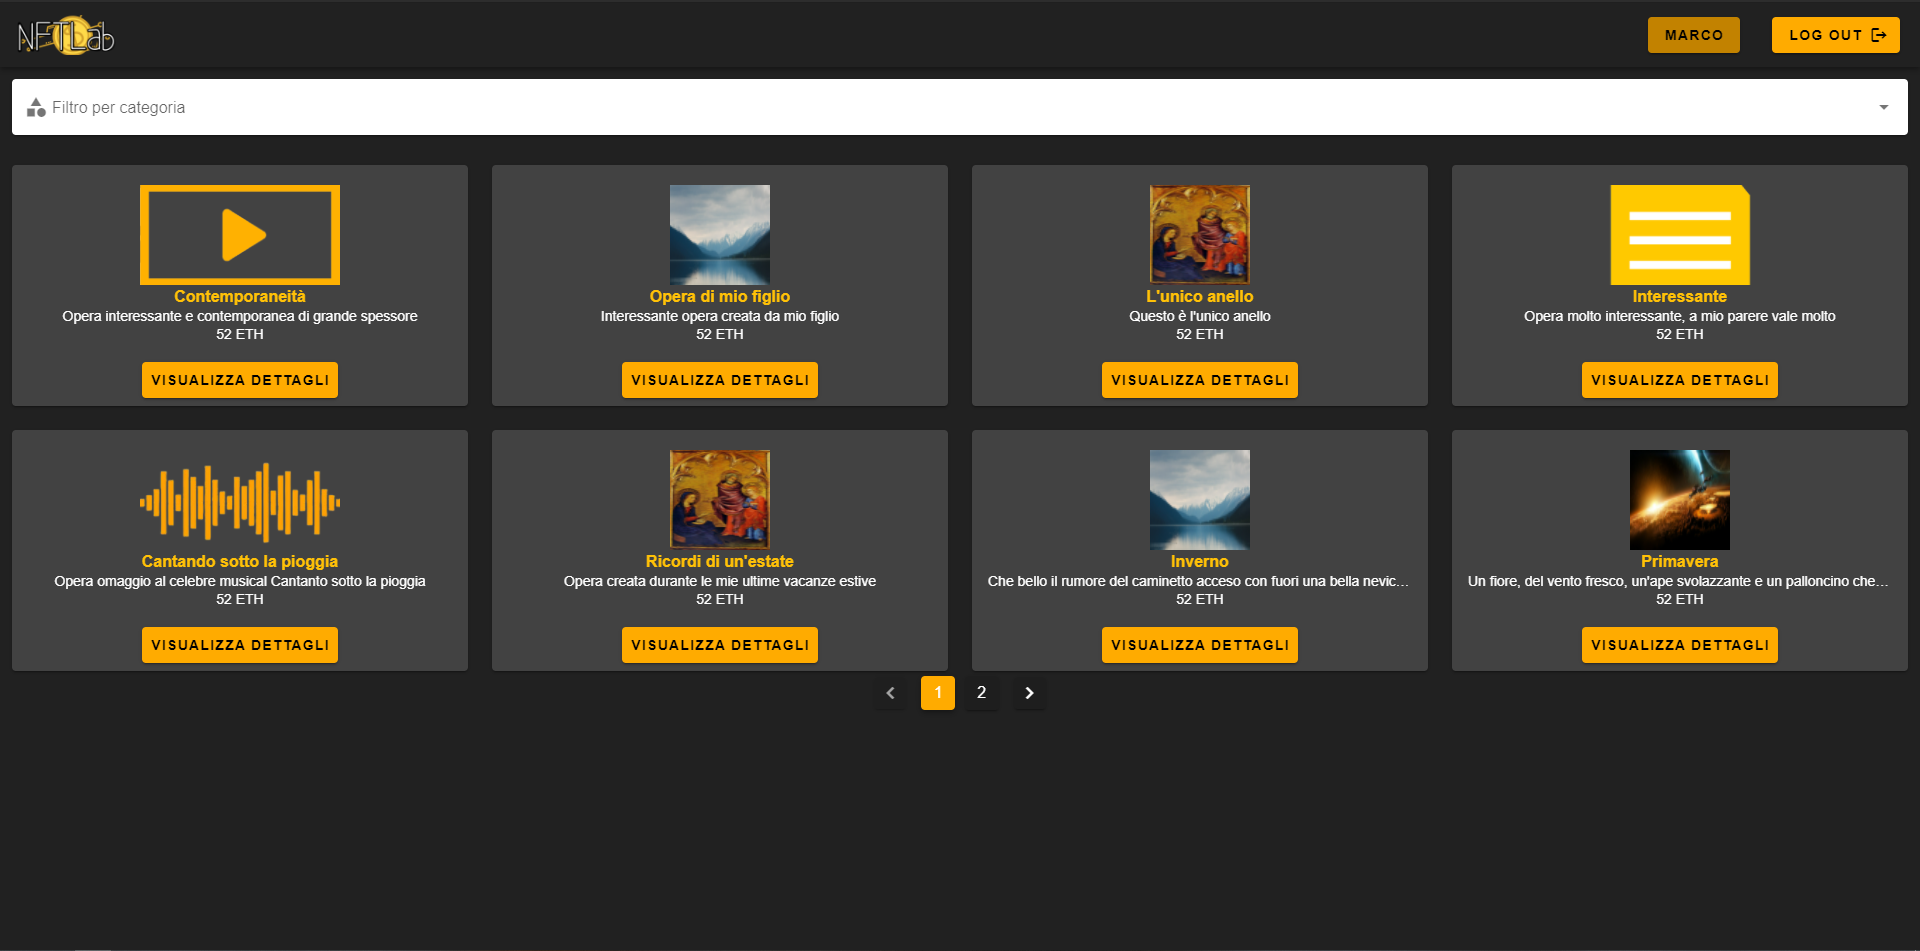
\includegraphics[width=0.9\columnwidth]{cap4/home.png}
		\caption{Home Page}
	\end{center}
\end{figure}

\subsection{Visualizza dettagli}
\label{subsec:visualizza-dettagli}

Questa funzionalità fa apparire una finestra di dialogo a schermo interno che mostra tutte le informazioni dettagliate dell'opera selezionata. Nella parte sinistra l'utente potrà vedere una preview dell'opera, mentre nella parte sinistra l'utente potrà vedere: titolo, prezzo con valuta, descrizione, autore, proprietario e categorie di appartenenza.
\begin{figure}[H]
	\begin{center}
		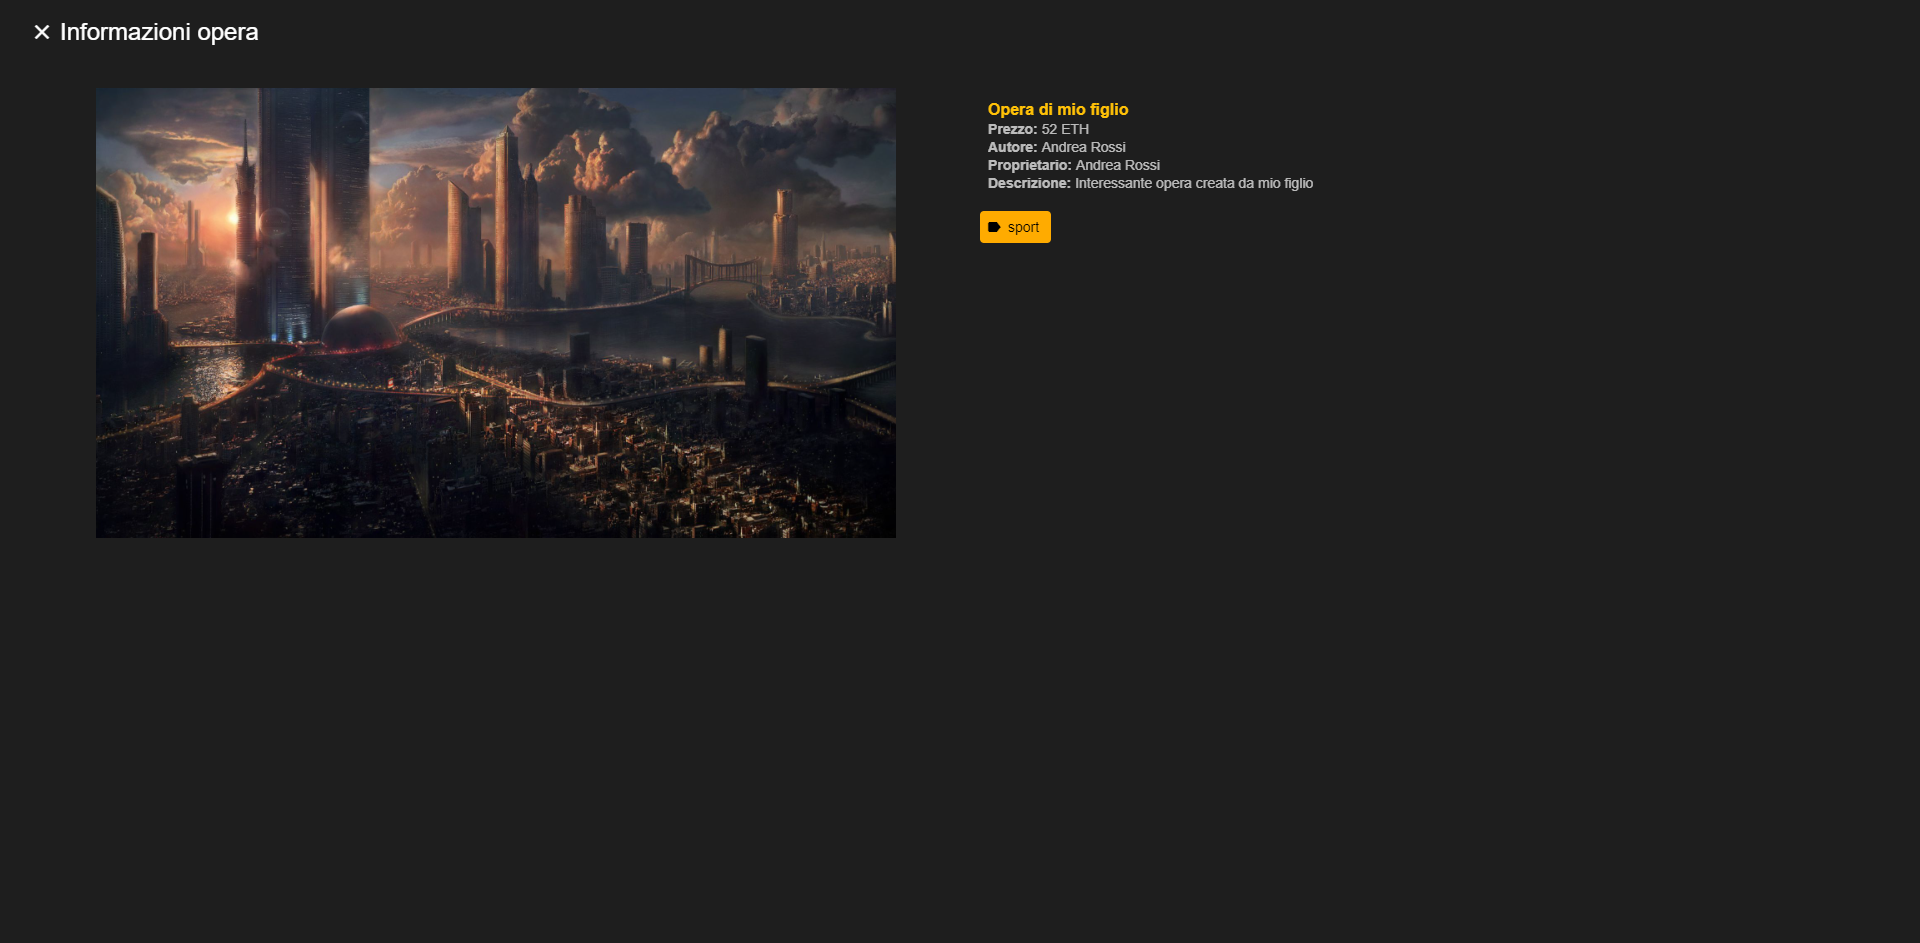
\includegraphics[width=0.9\columnwidth]{cap4/dettagliHome.png}
		\caption{Finestra di dialogo delle informazioni dell'opera}
	\end{center}
Questa finestra di dialogo è stata progettata a schermo intero in modo tale da poter aggiungere ulteriori informazioni o funzionalità senza dover modificare la struttura della finestra di dialogo.
\end{figure}

\subsection{Login}
\label{subsec:login}

In questa pagina l'utente può effettuare l'autenticazione nel sito tramite email e password. In questi due campi sono state inserite delle regole che, se non rispettate, generano un errore visualizzabile tramite una scritta sotto il campo che si sta modificando. Le regole in questione sono:
\begin{itemize}
	\item entrambi i campi sono obbligatori, quindi devono essere tutti compilati;
	\item l'email inserita deve essere valida\\
	\textit{esempio di email valida: nome@email.it};
	\item la password deve avere una lunghezza di minimo otto caratteri di cui almeno una lettera maiuscola, una minuscola, un numero e una carattere speciale.
\end{itemize}
\begin{figure}[H]
	\begin{center}
		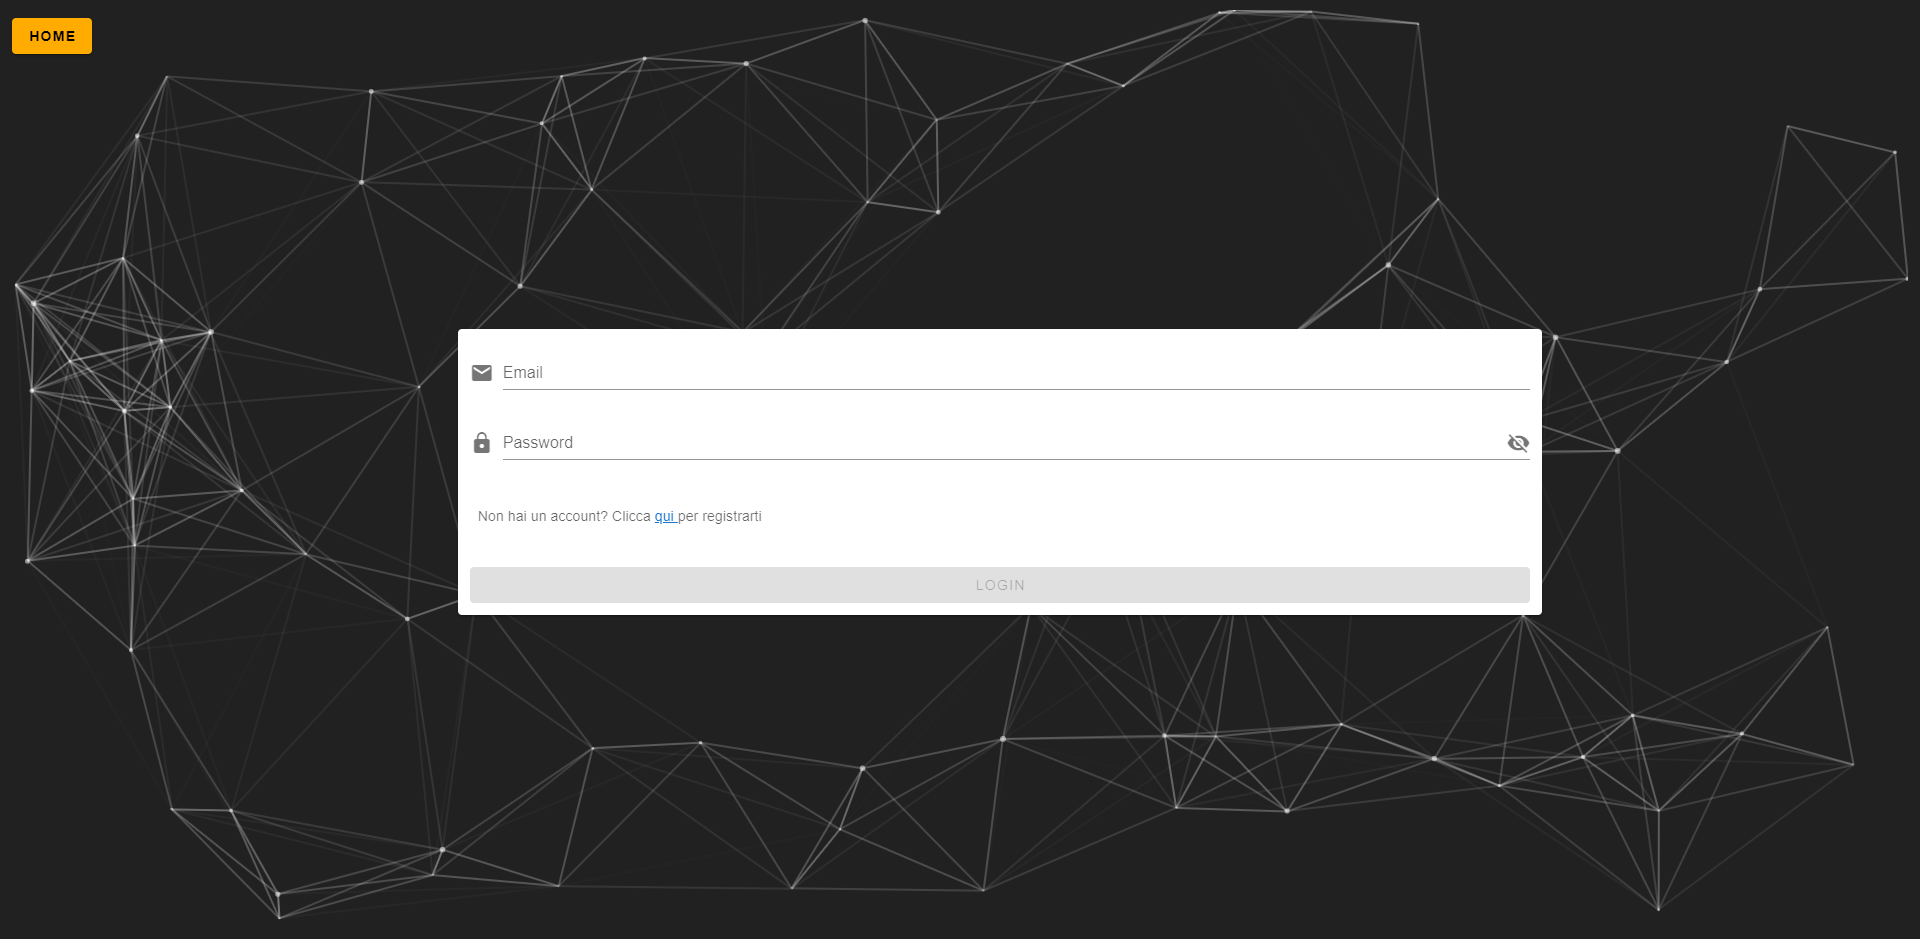
\includegraphics[width=0.9\columnwidth]{cap4/login.png}
		\caption{Pagina di login}
	\end{center}
\end{figure}
In alto a sinistra è presente un bottone per tornare alla home. Inoltre il bottone per validare l'autenticazione è disabilitato fino a quando l'utente non compila entrambi i campi per evitare chiamate al \gls{back endg} con dati mancanti.

\subsection{Registrazione}
\label{subsec:registrazione}

In questa pagine l'utente può effettuare la registrazione nel sito inserendo: nome, cognome, email, data di nascita, wallet address, password e conferma password. Similmente alla pagina di login sono state inserite delle regole che, se non rispettate, generano un errore visualizzabile tramite una scritta sotto il campo che si sta modificando. Le regole in questione sono:
\begin{itemize}
	\item tutti i campi sono obbligatori, quindi devono essere tutti compilati;
	\item l'email inserita deve essere valida\\
	\textit{esempio di email valida: nome@email.it};
	\item la data di nascita deve corrispondere ad una persona maggiorenne;
	\item il wallett address inserito deve essere valido\\ 
	\textit{esempio di wallett address valido: 0x390c7a1EA64e521B725b1869Ea054DDBF05F9abe};
	\item la password deve avere una lunghezza di minimo otto caratteri di cui almeno una lettera maiuscola, una minuscola, un numero e una carattere speciale;
	\item la conferma della password deve essere identica alla password appena inserita.
\end{itemize}
\begin{figure}[H]
	\begin{center}
		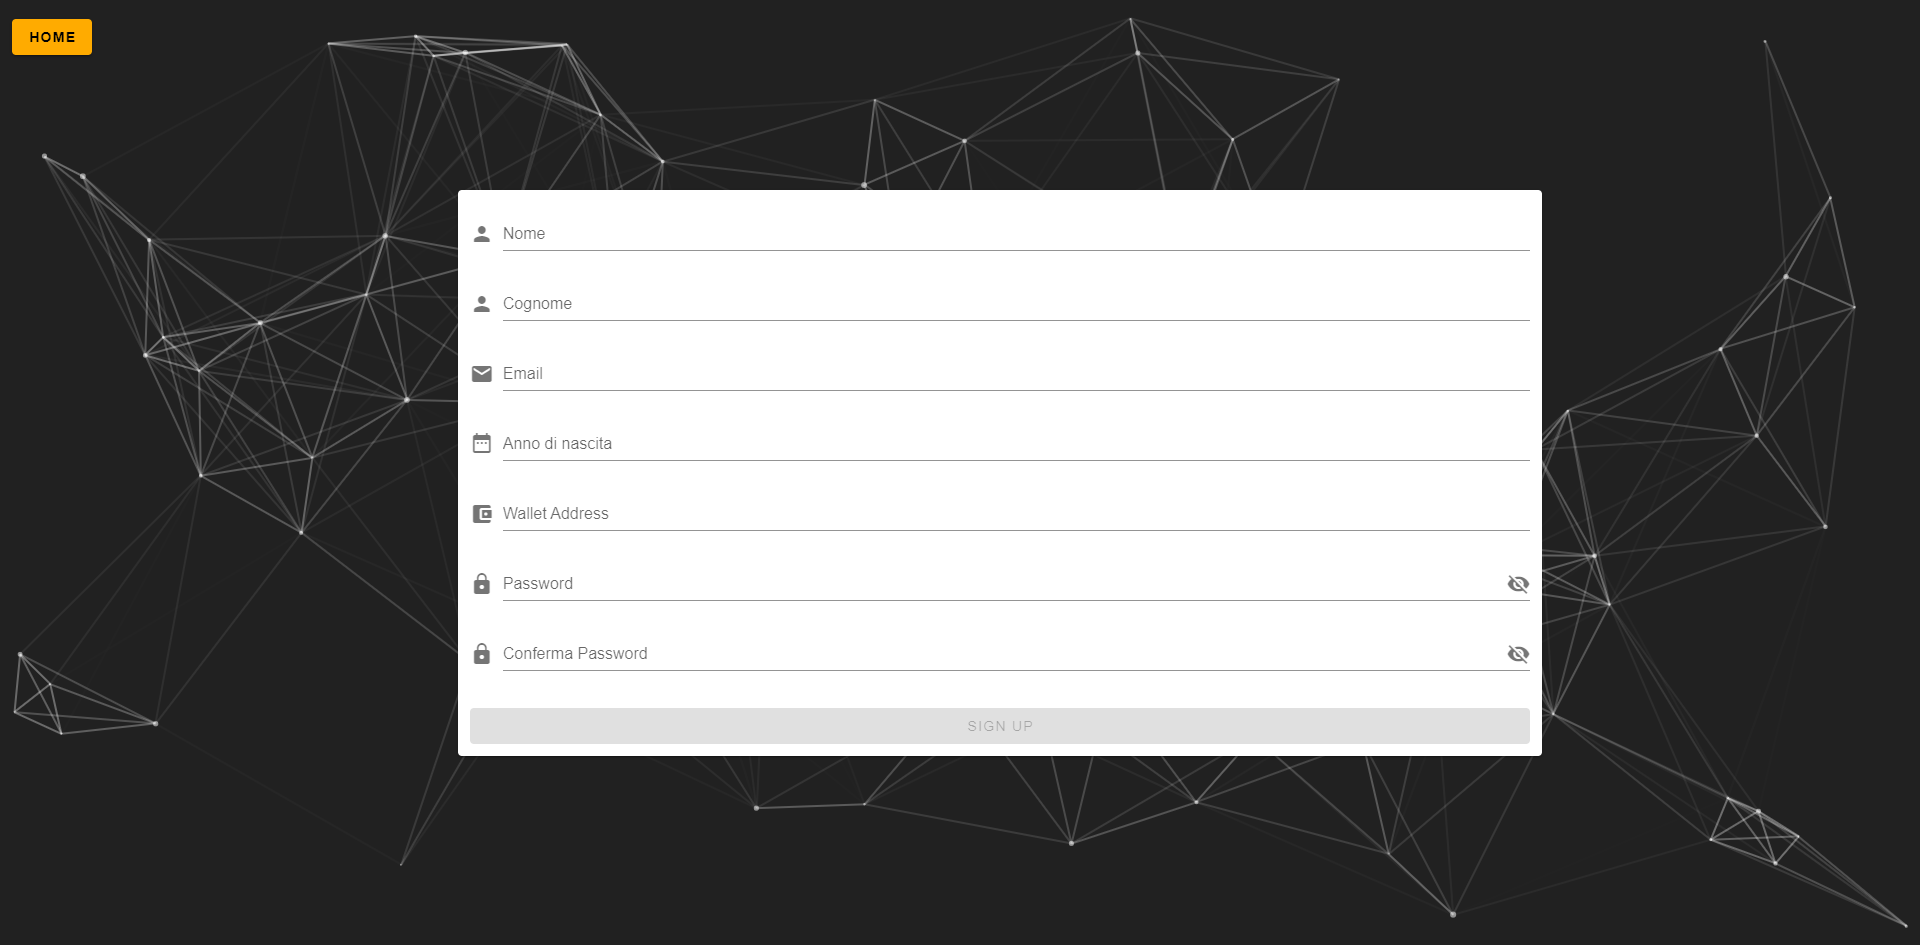
\includegraphics[width=0.9\columnwidth]{cap4/registrazione.png}
		\caption{Pagina di registrazione}
	\end{center}
\end{figure}
Come per la pagina di autenticazione, in alto a sinistra è presente un bottone per tornare alla home. Inoltre il bottone per validare l'autenticazione è disabilitato fino a quando l'utente non compila entrambi i campi per evitare chiamate al \gls{back endg} con dati mancanti.

\subsection{Pagina dell'utente}
\label{subsec:pagina-utente}

In questa pagina l'utente può visualizzare le sue informazioni personali e le opere che possiede. Nel momento che verranno modificate le informazioni da parte dell'utente, queste verranno modificate a schermo automaticamente.
\begin{figure}[H]
	\begin{center}
		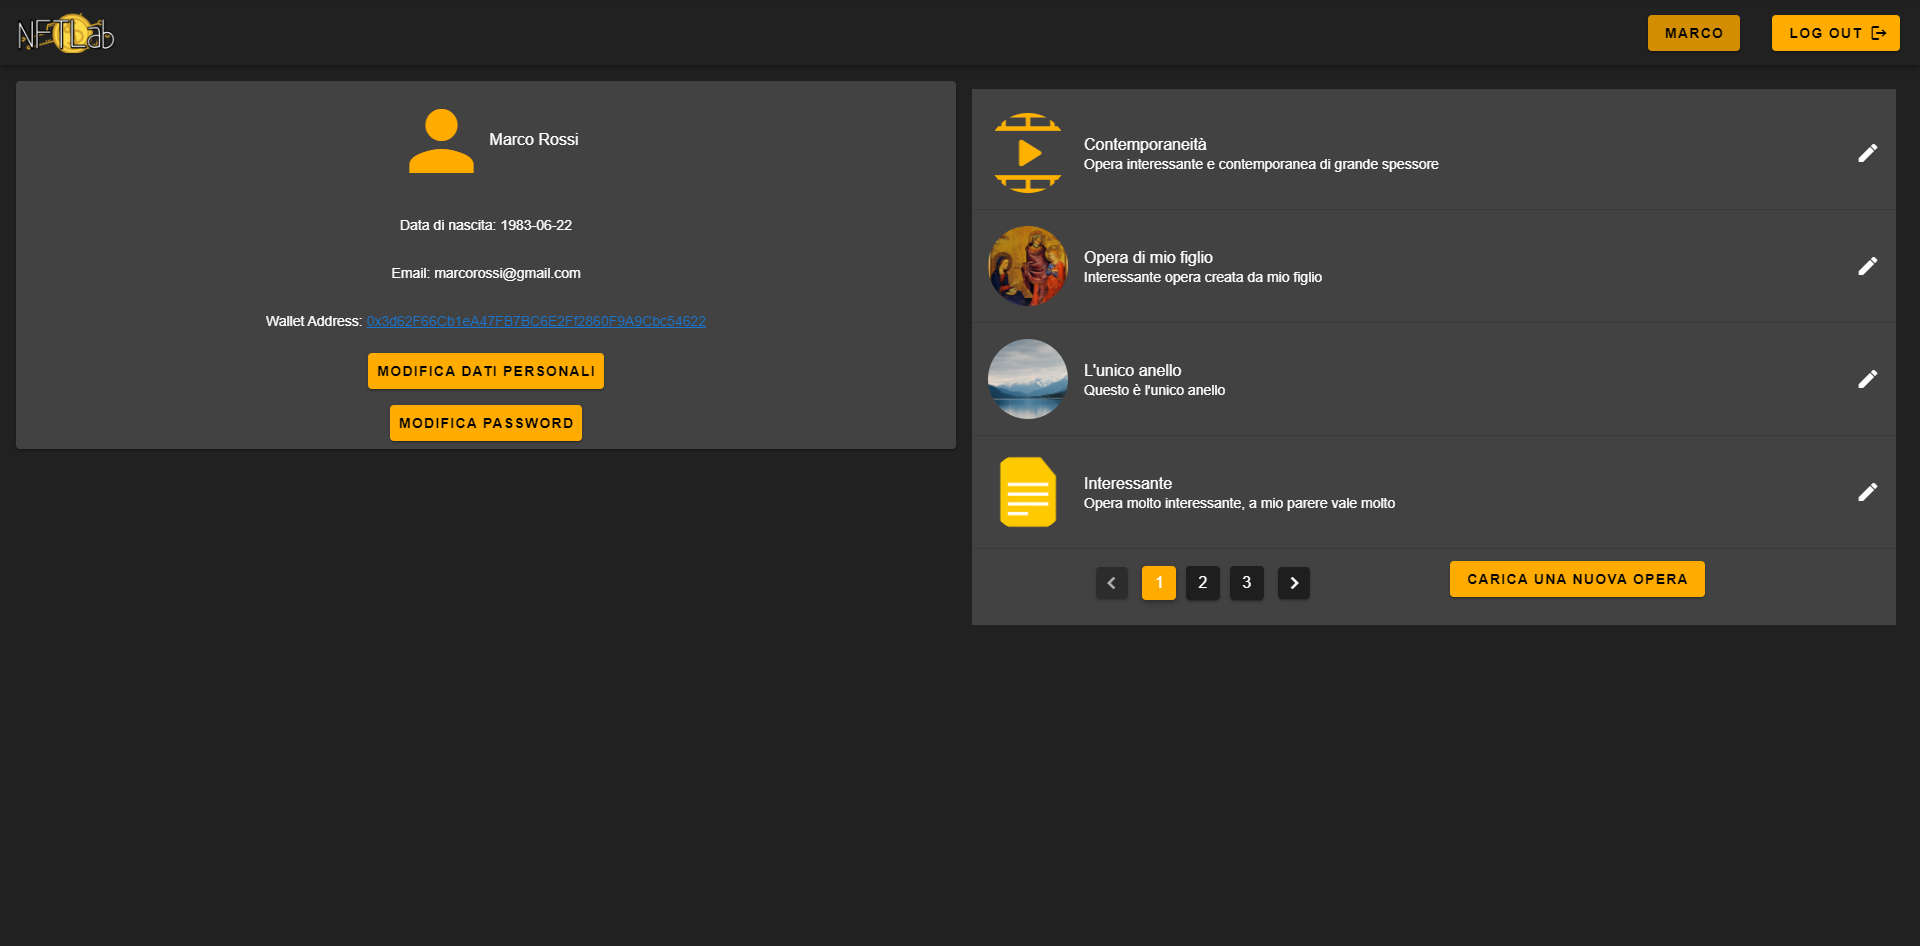
\includegraphics[width=0.9\columnwidth]{cap4/userPage.png}
		\caption{Pagina personale dell'utente}
	\end{center}
\end{figure}

\subsection{Upload opera}
\label{subsec:upload-opera}

In questa pagina è possibile per l'utente aggiungere una nuova opera. I campi da compilare sono: titolo, descrizione, file, prezzo. Quando l'utente carica un file verranno generati automaticamente una preview del file specifica in base al tipo del file inserito e un campo non modificabile che indica il tipo del file inserito. Similmente alla pagina di registrazione sono state inserite delle regole che, se non rispettate, generano un errore visualizzabile tramite una scritta sotto il campo che si sta modificando. Le regole in questione sono:
\begin{itemize}
	\item tutti i campi sono obbligatori, quindi devono essere tutti compilati.
\end{itemize}
\begin{figure}[H]
	\begin{center}
		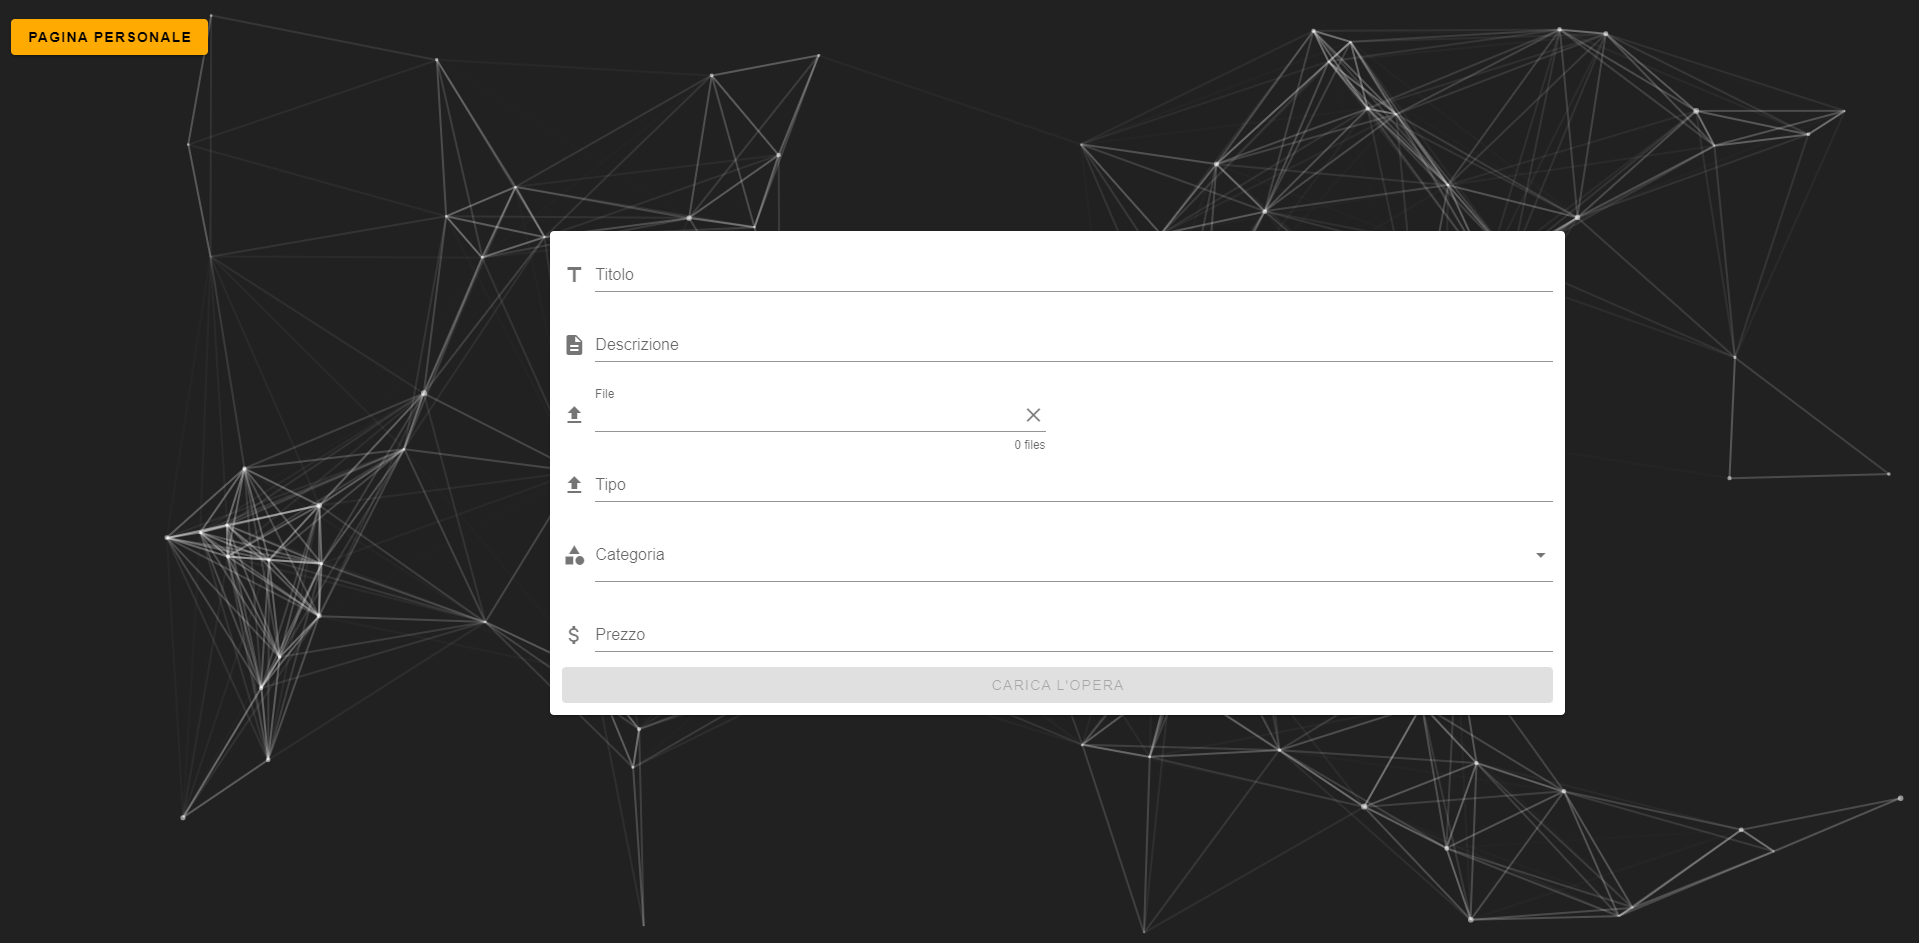
\includegraphics[width=0.9\columnwidth]{cap4/uploadOpera.png}
		\caption{Pagina di upload dell'opera}
	\end{center}
\end{figure}
Nel momento in cui l’utente carica il file verrà aggiornato automaticamente il campo legato alla tipologia di file.
Questo campo non `e modificabile da parte dell'utente.
\subsection{Gestione opere}
\label{subsec:gestione-opere}

L'utente può unicamente modificare una sua opera ma non può cancellarla. Questo è dovuto al fatto che al momento dell'upload l'opera verrà caricata sulla blockchain rendendola un elemento unico ed irripetibile quindi non può cancellarla. Per motivi analoghi l'utente ha delle restrizioni anche nella modifica dell'opera; infatti di essa può modificare solo: titolo, descrizione, prezzo e categorie di appartenenza. Un altro campo non modificabile è il tipo del file caricato.
\begin{figure}[H]
	\begin{center}
		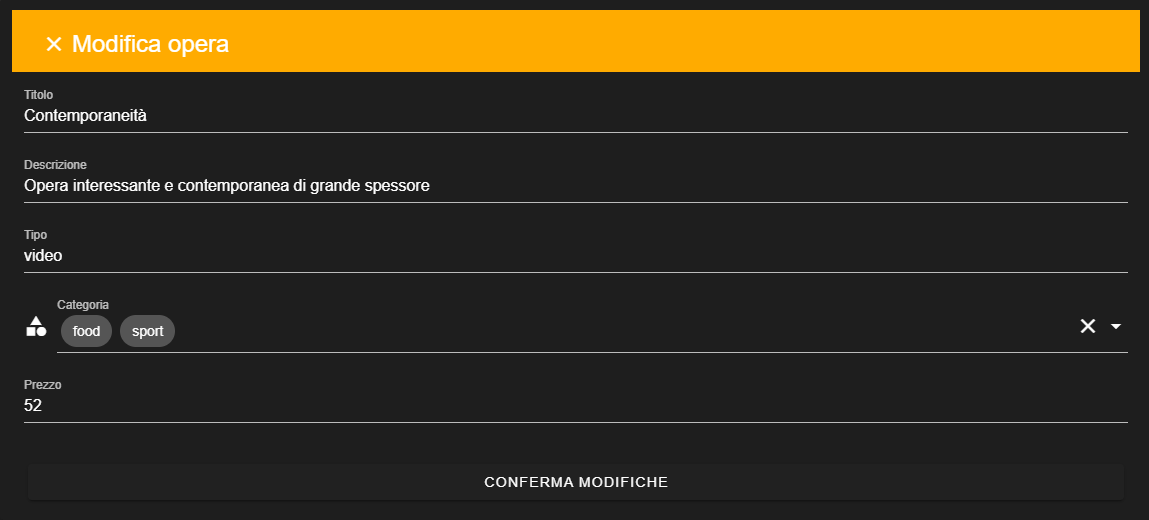
\includegraphics[width=0.9\columnwidth]{cap4/modificaOpera.png}
		\caption{Finestra di dialogo per la modifica dell'opera}
	\end{center}
\end{figure}

\subsection{Modifica dati personali}
\label{subsec:modifica-dati-personali}

L'utente, dopo aver premuto un bottone con la dicitura "Modifica dati personali", vedrà apparire una finestra di avviso dove può modificare i propri dati. Per motivi di univocità l'utente non potrà modificare l'email con cui ha fatto l'accesso, infatti potrà modificare solamente il nome ed il cognome. Inoltre per motivi di sicurezza il bottone per confermare la modifica è disabilitato di default e viene data la possibilità di confermare la modifica solo dopo aver inserito la password corrente.
\begin{figure}[H]
	\begin{center}
		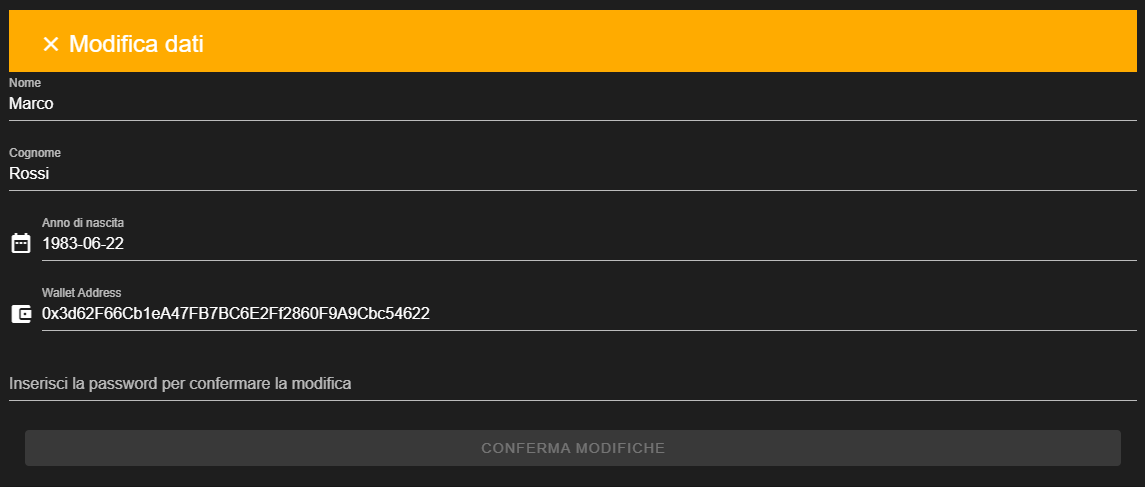
\includegraphics[width=0.8\columnwidth]{cap4//modificaDati.png}
		\caption{Finestra di dialogo per la modifica dei dati}
	\end{center}
\end{figure}

\subsection{Modifica password}
\label{subsec:modifica-password}

L'utente dopo aver premuto un bottone con la dicitura "Modifica password", vedrà apparire una finestra di avviso dove può modificare la password. Per poterlo fare, per motivi di sicurezza, l'utente dovrà inserire la sua email, la password corrente e la nuova password. Similmente alla modifica dei dati personali, il bottone per confermare la modifica rimarrà disattivato fino a quando l'utente non avrà completato tutti i campi.
\begin{figure}[H]
	\begin{center}
		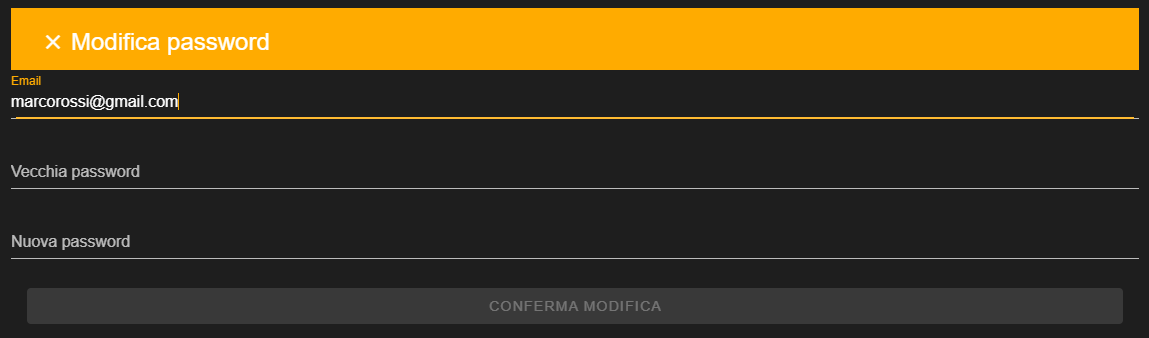
\includegraphics[width=0.8\columnwidth]{cap4/modificaPassword.png}
		\caption{Finestra di dialogo per la modifica della password}
	\end{center}
\end{figure}

\section{Generazione della preview}
\label{sec:generazione-preview}

Per quanto riguarda le immagini presenti nella home page, nella pagina dell'utente e nelle finestre di dialogo che mostrano i dettagli dell'opera, viene generata una preview in base alla tipologia del file. Infatti se il tipo del file è un immagine si potrà visualizzare una preview effettiva di essa, altrimenti se il tipo del file è audio, video o documento verranno visualizzate delle immagini preimpostate che fanno intuire la tipologia del file.\\
Questo ragionamento viene applicato anche quando l'utente carica una nuova opera. Infatti nel momento in cui l'utente seleziona un file verrà mostrata una preview generata utilizzando il ragionamento appena descritto.